\section{Análisis}

\subsection{Listado de todas las publicaciones de un autor determinado.}

Para esta query vamos a hacer uso de la potencia que nos ofrece el \textit{aggregation framework}. Este framework funciona creando un pipeline en la que definiremos \textit{stages}. La salida de un \textit{stage} pasa a ser la entrada del \textit{stage} siguiente. Con esto podemos realizar sobre los datos operaciones realmente potentes.

Para obtener el listado de las publicaciones, la query que debemos ejecutar es sencilla. En primer lugar filtramos por el nombre de autor que del cual queremos hacer la consulta, y a continuación concatenamos los \textit{arrays} con los títulos de las publicaciones.

\begin{minted}[
frame=single]{js}
db.authors.aggregate([
  { $match : { _id : "Chin-Wang Tao" } }, 
  { $project: {publication: {$concatArrays: 
    ["$incollections.title", "$articles.title", "$inproceedings.title"]}}
  }
] )
\end{minted}


Como resultado obtenemos:

\begin{minted}[
frame=single,breaklines]{js}
/* 1 */
{
    "_id" : "Chin-Wang Tao",
    "publication" : [ 
        "iPhone as Multi-CAM and Multi-viewer.", 
        "On the robustness of stability of fuzzy control systems.", 
        "Adaptive fuzzy PIMD controller for systems with uncertain deadzones.", 
        "Design and analysis of region-wise linear fuzzy controllers.", 
        "Adaptive Fuzzy Switched Swing-Up and Sliding Control for the Double-Pendulum-and-Cart System.", 
        "An Approximation of Interval Type-2 Fuzzy Controllers Using Fuzzy Ratio Switching Type-1 Fuzzy Controllers.", 
        "Adaptive fuzzy terminal sliding mode controller for linear systems with mismatched time-varying uncertainties.", 
        "A reduction approach for fuzzy rule bases of fuzzy controllers.", 
        "Fuzzy Sliding-Mode Formation Control for Multirobot Systems: Design and Implementation.", 
        "Segmentation of Psoriasis Vulgaris Images Using Multiresolution-Based Orthogonal Subspace Techniques.", 
        "Fuzzy control for linear plants with uncertain output backlashes.", 
        "Iris Recognition Using Possibilistic Fuzzy Matching on Local Features.", 
        "Radial Basis Function Networks With Linear Interval Regression Weights for Symbolic Interval Data.", 
        "Adaptive fuzzy sliding mode controller for linear systems with mismatched time-varying uncertainties.", 
        "Design of fuzzy controllers with adaptive rule insertion.", 
        "Flexible complexity reduced PID-like fuzzy controllers.", 
        "Interval competitive agglomeration clustering algorithm.", 
        "Fuzzy sliding-mode control for ball and beam system with fuzzy ant colony optimization.", 
        "Hybrid robust approach for TSK fuzzy modeling with outliers.", 
        "Design of a Fuzzy Controller With Fuzzy Swing-Up and Parallel Distributed Pole Assignment Schemes for an Inverted Pendulum and Cart System.", 
        "Nested design of fuzzy controllers with partial fuzzy rule base.", 
        "Fuzzy hierarchical swing-up and sliding position controller for the inverted pendulum-cart system.", 
        "Design of a parallel distributed fuzzy LQR controller for the twin rotor multi-input multi-output system.", 
        "Fuzzy adaptive approach to fuzzy controllers with spacial model.", 
        "Simplified type-2 fuzzy sliding controller for wing rock system.", 
        "Unsupervised fuzzy clustering with multi-center clusters.", 
        "An advanced fuzzy controller.", 
        "A Novel Approach to Implement Takagi-Sugeno Fuzzy Models.", 
        "Fuzzy Swing-Up and Fuzzy Sliding-Mode Balance Control for a Planetary-Gear-Type Inverted Pendulum.", 
        "A Design of a DC-AC Inverter Using a Modified ZVS-PWM Auxiliary Commutation Pole and a DSP-Based PID-Like Fuzzy Control.", 
        "Robust fuzzy control for a plant with fuzzy linear model.", 
        "Comments on \"Reduction of fuzzy rule base via singular value decomposition\".", 
        "A Novel Fuzzy-Sliding and Fuzzy-Integral-Sliding Controller for the Twin-Rotor Multi-Input-Multi-Output System.", 
        "Robust L", 
        "A Fuzzy Logic Approach to Target Tracking", 
        "Index compression for vector quantisation using modified coding tree assignment scheme.", 
        "Hybrid SVMR-GPR for modeling of chaotic time series systems with noise and outliers.", 
        "Parallel Distributed Fuzzy Sliding Mode Control for Nonlinear Mismatched Uncertain Systems.", 
        "An approach for the robustness comparison between piecewise linear ", 
        "Interval fuzzy sliding-mode formation controller design.", 
        "Simplification of a fuzzy mechanism with rule combination.", 
        "Robust control of systems with fuzzy representation of uncertainties.", 
        "Checking identities is computationally intractable NP-hard and therefore human provers will always be needed.", 
        "A kernel-based core growing clustering method.", 
        "An Alternative Type Reduction Approach Based on Information Combination with Interval Operations for Interval-Valued Fuzzy Sliding Controllers.", 
        "Designs and analyses of various fuzzy controllers with region-wise linear PID subcontrollers.", 
        "Adaptive Bound Reduced-Form Genetic Algorithms for B-Spline Neural Network Training.", 
        "A New Neuro-Fuzzy Classifier with Application to On-Line Face Detection and Recognition.", 
        "Statistical and Dempster-Shafer Techniques in Testing Structural Integrity of Aerospace Structures.", 
        "Embedded support vector regression on Cerebellar Model Articulation Controller with Gaussian noise.", 
        "Iris Recognition Using Gabor Filters and the Fractal Dimension.", 
        "A two-stage design of adaptive fuzzy controllers for time-delay systems with unknown models.", 
        "Errata: Iris recognition using Gabor filters optimized by the particle swarm algorithm.", 
        "Texture classification using a fuzzy texture spectrum and neural networks.", 
        "Iris recognition using Gabor filters optimized by the particle swarm algorithm.", 
        "Sliding control for linear uncertain systems.", 
        "FPGA implementation of improved ant colony optimization algorithm for path planning.", 
        "Medical image compression using principal component analysis.", 
        "Design of a Kinect Sensor Based Posture Recognition System.", 
        "A simplified interval type-2 fuzzy CMAC.", 
        "iOS based Multi-Cloud Manage System.", 
        "A Novel Approach to Implement Takagi-Sugeno Fuzzy Models.", 
        "Path-planning using the behavior cost and the path length with a multi-resolution scheme.", 
        "Iris recognition using Gabor filters optimized by the particle swarm technique.", 
        "Hybrid robust LS-SVMR with outliers for MIMO system.", 
        "Design of A Two-Stage Adaptive Fuzzy Controller.", 
        "Face Detection Using Eigenface and Neural Network.", 
        "Robust control of the mismatched systems with the fuzzy integral sliding controller.", 
        "Support Vector Regression for Controller Approximation.", 
        "Robust clustering algorithm for the symbolic interval-values data with outliers."
    ]
}
\end{minted}


\subsection{Número de publicaciones de un autor determinado.}

Esta consula es similar a la anterior, pero debemos añadir un paso más en nuestro \textit{pipeline} en el cual contaremos el número de puclicaciones.

\begin{minted}[
frame=single]{js}
db.authors.aggregate([
  { $match : { _id : "Chin-Wang Tao" } }, 
  { $project: {publications: {$concatArrays: 
    ["$incollections.title", "$articles.title", "$inproceedings.title"]}}
  },
  {$project: {number_of_publications: {$size: "$publications"}}}
] )
\end{minted}


Como resultado obtenemos:

\begin{minted}[
frame=single]{js}
/* 1 */
{
    "_id" : "Chin-Wang Tao",
    "number_of_publications" : 70
}
\end{minted}

\subsection{Número de artículos en revistas para el año 2017.}

\begin{minted}[
frame=single]{js}
db.articles.find({year: 2017}).count()
\end{minted}

Aprovechando que esta query es simple, podemos ver la importancia que adquieren los índices en cuanto a tiempo de ejecución. Para ello, generamos el índice sobre el campo year de la siguiente forma:

\begin{minted}[
frame=single]{js}
db.articles.createIndex({year:1})
\end{minted}


\begin{minted}[
frame=single]{js}
/* 1 */
{
    "createdCollectionAutomatically" : false,
    "numIndexesBefore" : 1,
    "numIndexesAfter" : 2,
    "ok" : 1.0
}
\end{minted}

Vemos que el resultado es satisfactorio y que a partir de este momento, además del índice originario (sobre \_id), tenemos índice sobre year.

La comparativa en tiempos de ejecución es la siguiente:

\begin{figure}[H]
  \centering
    \centering
        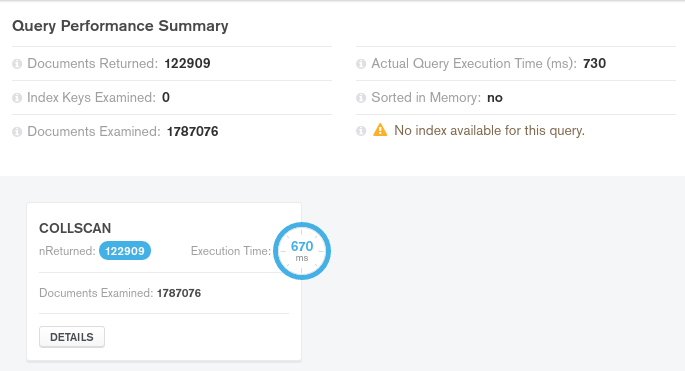
\includegraphics[width=0.4\textwidth]{Figures/wo_year_idx}
        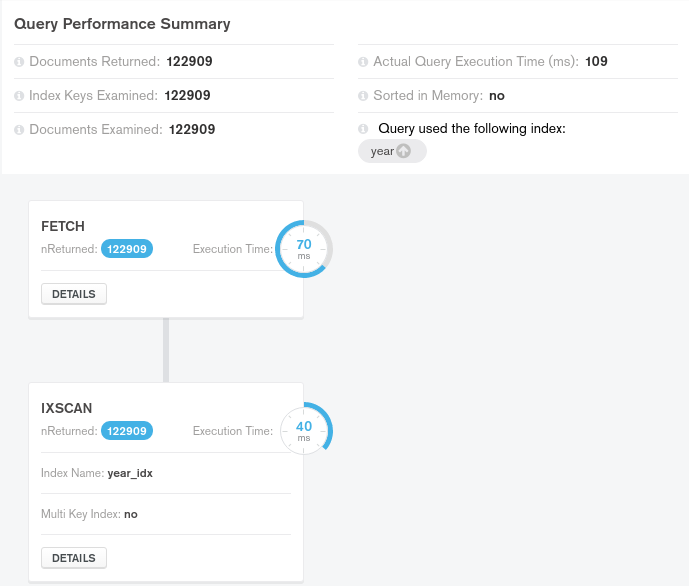
\includegraphics[width=0.4\textwidth]{Figures/year_idx}
  \caption{A la izquierda, la query sin índice, a la derecha, aplicando un índice sobre la columna year.}
\end{figure}

El tiempo de respuesta es casi 7 veces inferior al hacer uso del índice.

Como resultado, independientemente del uso de índice, obtenemos:

\begin{minted}[
frame=single]{js}
136121
\end{minted}

\subsection{Número de autores ocasionales (menos de 5 publicaciones).}

En esta ocasión no hará falta hacer uso del \textit{aggregation framework}, si no que haremos una búsqueda utilizando la función \textbf{find()}.

\begin{minted}[
frame=single]{js}
db.authors.find({$expr: {$lt: [{$concatArrays: ["$incollections", "$articles",
  "$inproceedings"]}, 5]}}).count()
\end{minted}


Como resultado obtenemos:

\begin{minted}[
frame=single]{js}
1988889
\end{minted}

\subsection{Número de artículos y de artículos en congresos de los diez autores con más publicaciones en total.}

Volvemos a usar \textit{aggregation framework} y construimos un \textit{pipeline} con varios pasos. Primero contamos el número de cada tipo de publicacion de cada uno de los autores. A continuación, creamos un nuevo campo con el con \textbf{\$addFields} con el total de publicaciones. Con \textbf{\$sort} y \textbf{\$limit} ordenamos por el campo recién creado y nos quedamos solo con los 10 primeros, es decir, con los autores que más publicaciones tienen. Por último, y con el \textit{stage} \textbf{\$project}, nos quedamos solo con los campos que nos interesan (el campo \textbf{\_id} se incluye por defecto si no se especifica lo contrario).

\begin{minted}[
frame=single]{js}
db.authors.aggregate(
  [
    {$project: {
      "total_incollections": {$size: {$ifNull: ['$incollections', []]},},
      "total_inproceedings": {$size: {$ifNull: ['$inproceedings', []]},},
      "total_articles": {$size: {$ifNull: ['$articles', []]},}
    }},
    {$addFields: {
      "total_publications": { $add: [ "$total_incollections", "$total_inproceedings",
                  "$total_articles" ] }
    }},
    {$sort : { total_publications : -1 } },
    {$limit : 10},
    {$project: {
      "total_articles": 1,
      "total_inproceedings": 1
    }}
  ],
  { allowDiskUse: true }
)
\end{minted}

Como resultado obtenemos:

\begin{minted}[
frame=single]{js}
/* 1 */
{
    "_id" : "H. Vincent Poor",
    "total_inproceedings" : 477,
    "total_articles" : 1024
}

/* 2 */
{
    "_id" : "Mohamed-Slim Alouini",
    "total_inproceedings" : 533,
    "total_articles" : 600
}

/* 3 */
{
    "_id" : "Philip S. Yu",
    "total_inproceedings" : 707,
    "total_articles" : 389
}

/* 4 */
{
    "_id" : "Wen Gao 0001",
    "total_inproceedings" : 734,
    "total_articles" : 332
}

/* 5 */
{
    "_id" : "Wei Wang",
    "total_inproceedings" : 630,
    "total_articles" : 430
}

/* 6 */
{
    "_id" : "Yu Zhang",
    "total_inproceedings" : 616,
    "total_articles" : 429
}

/* 7 */
{
    "_id" : "Lajos Hanzo",
    "total_inproceedings" : 407,
    "total_articles" : 635
}

/* 8 */
{
    "_id" : "Wei Li",
    "total_inproceedings" : 554,
    "total_articles" : 449
}

/* 9 */
{
    "_id" : "Li Zhang",
    "total_inproceedings" : 577,
    "total_articles" : 404
}

/* 10 */
{
    "_id" : "Yang Liu",
    "total_inproceedings" : 553,
    "total_articles" : 417
}
\end{minted}

\subsection{Número medio de autores por publicación.}

En este caso vamos a tener que hacer consulta a varias coleciones y luego hacer calculos con los datos obtenidos en estas consultas.

En primer lugar realizamos consultas en cada una de las colecciones para obtener el número total de autores, incluyendo duplicados. Es decir, si por ejemplo, en un artículo han participado 3 autores, se sumara 3 a la cuenta de autores para esta colección. Estos resultados son sumados y el total lo dividimos por el número total de publicaciones guardadas.

\begin{minted}[
frame=single]{js}
(db.articles.aggregate([
  {$match: {author : {$exists: true}}}, 
  {$project: {num_authors: { $size: '$author' }}}, 
  {$group: {_id: '', num_authors: {$sum: '$num_authors'}}}, 
  {$project: {_id: 0, 'num_authors': '$num_authors'}}])
  .next()['num_authors'] +
db.incollections.aggregate([
  {$match: {author : {$exists: true}}}, 
  {$project: {num_authors: { $size: '$author' }}}, 
  {$group: {_id: '', num_authors: {$sum: '$num_authors'}}}, 
  {$project: {_id: 0, 'num_authors': '$num_authors'}}])
  .next()['num_authors'] +
db.inproceedings.aggregate([
  {$match: {author : {$exists: true}}}, 
  {$project: {num_authors: { $size: '$author' }}}, 
  {$group: {_id: '', num_authors: {$sum: '$num_authors'}}}, 
  {$project: {_id: 0, 'num_authors': '$num_authors'}}])
  .next()['num_authors'])/
(db.articles.find().count() + 
  db.incollections.find().count() + 
  db.inproceedings.find().count())
\end{minted}

Como resultado obtenemos:

\begin{minted}[
frame=single]{js}
2.947463651066849
\end{minted}

\subsection{Lista de coautores de un autor.}

Para poder recuperar esta información, será necesario acceder a cada una de las publicaciones de la lista de publicaciones de un autor, ``seguir'' la referencia para obtener la publicación, y extraer los autores de esta. Para poder ``seguir'' una referencia a otro documento, \textit{aggregation framework} cuenta con el \textit{stage} \textbf{\$lookup}, al que le decimos en que colección buscar y que campos tiene que utilizar a la hora de realizar la busqueda.

\begin{minted}[
frame=single]{js}
db.authors.aggregate([
  { $match : { _id : "Chin-Wang Tao" } },
  {$lookup:
    {
      from: "articles",
      localField: "articles._id",
      foreignField: "_id",
      as: "articles_detail"
    }
  },
  {$lookup:
    {
      from: "incollections",
      localField: "incollections._id",
      foreignField: "_id",
      as: "incollections_detail"
    }
  },
  {$lookup:
    {
      from: "inproceedings",
      localField: "inproceedings._id",
      foreignField: "_id",
      as: "inproceedings_detail"
    }
  },
  {$project:{
      _id : 1,
      authors_detail : { $concatArrays: [ "$articles_detail", "$incollections_detail", "$inproceedings_detail" ] }
    } 
  },
  {$project: {
    "_id": 0,
    "results": {
      $reduce: {
        input: "$authors_detail.author",
        initialValue: [],
        in: { $concatArrays : ["$$value", "$$this"] }
      }
    }
  }
  },
  { $unwind : "$results" },
  {$group: {
    _id: "$results",
    }
  },
  {$group: {
      _id: null,
      coauthors: { $push: { _id: "$_id"} }
    }
  },
  {$project: {
      _id: 0,
      "coauthors": "$coauthors._id"
    }
  }
])
\end{minted}


Como resultado obtenemos:

\begin{minted}[
frame=single]{js}
/* 1 */
{
    "coauthors" : [ 
        "T. H. Su", 
        "W. C. Cheng", 
        "C. C. Tsai", 
        "Meng-Hua Lai", 
        "W. Z. Chen", 
        "Po-Chun Wang", 
        "Song-Shyong Chen", 
        "Wen-Rong Xiao", 
        "Tzuen Wuu Hsieh", 
        "Jin-Tsong Jeng", 
        "Hung-Wei Lin", 
        "Gwo-Her Lee", 
        "Tsu-Tian Lee", 
        "Ching-Wen Yang", 
        "Chia-Chu Hsu", 
        "Ze-Si Huang", 
        "Chung-Chih Tsai", 
        "Chin-Wang Tao", 
        "Min Da Nian", 
        "Chien-Chou Chen", 
        "Heng-Yi Lin", 
        "Mei-Lang Chan", 
        "C. L. Tsai", 
        "Jin-Shiuh Taur", 
        "Jyun-Long Wu", 
        "Chia-Wen Chang", 
        "Chen-Guan Chang", 
        "Chen-Chien J. Hsu", 
        "Yeong-Hwa Chang", 
        "Chunlin Chen", 
        "Ching Ho Chi", 
        "Huei-Rong Chen", 
        "Chen-Chia Chuang", 
        "W. Y. Wang", 
        "Shun-Feng Su", 
        "Yi-Fang Chen", 
        "Rustom Mamlook", 
        "Meng-Cheng Yang", 
        "J. H. Chang", 
        "Y. C. Chen", 
        "Chien-Ming Wang", 
        "Yung-Chih Liu", 
        "U. S. Chen", 
        "Ana C. Holguin", 
        "Yao-Chu Hsueh", 
        "Sun-Yuan Kung", 
        "Cheng-Yuan Yang", 
        "C. M. Wang", 
        "Vladik Kreinovich", 
        "Wei-Yen Wang", 
        "Chih-Ching Hsiao", 
        "Roberto A. Osegueda", 
        "Seetharami R. Seelam", 
        "Yi-Hsing Chien", 
        "Wiley E. Thompson", 
        "Hung T. Nguyen 0002", 
        "Ru-Yu Hou"
    ]
}
\end{minted}

\subsection{Edad de los 5 autores con el periodo de publicaciones más largo.}

En primer lugar, y usando las facilidades de  \textit{aggregation framework}, agrupamos todas las publicaciones de un mismo autor en una lista única. A continuación nos quedamos de estas listas solo con el año de publicación de estas, y filtramos tanto el máximo como el mínimo de de estos años. Ya con esto, podemos calcular la diferencia entre ambos años y realizar una ordenación a partir de este campo para quedarnos con los cinco primeros.

\begin{minted}[
frame=single]{js}
db.authors.aggregate(
  [
    {$project: {
      publication: {$concatArrays: [
        {$ifNull: ['$incollections', []]},
        {$ifNull: ['$inproceedings', []]},
        {$ifNull: ['$articles', []]}]}
    }},
    {$addFields: {
      max_publication: { $max: "$publication.year"},
      min_publication: { $min: "$publication.year"}
    }},
    {$addFields: {
      age: { $subtract: [ "$max_publication", "$min_publication"] }
    }},
    {$sort : { age : -1 } },
    {$limit : 5},
    {$project: {
      _id: 1,
      age: 1
    }}
  ],
  { allowDiskUse: true }
)
\end{minted}


Como resultado obtenemos:

\begin{minted}[
frame=single]{js}
/* 1 */
{
    "_id" : "Alan M. Turing",
    "age" : 75
}

/* 2 */
{
    "_id" : "Rudolf Carnap",
    "age" : 71
}

/* 3 */
{
    "_id" : "David Nelson",
    "age" : 68
}

/* 4 */
{
    "_id" : "Eric Weiss",
    "age" : 64
}

/* 5 */
{
    "_id" : "Bernard Widrow",
    "age" : 64
}
\end{minted}

\subsection{Número de autores novatos.}

Caso idéntico al anterior, cambiando las fases finales para quedarnos con aquellos cuya ``edad'' es inferior a 5 años, y contar el número de elementos que obtenemos.

\begin{minted}[
frame=single]{js}
db.authors.aggregate(
  [
    {$project: {
      publication: {$concatArrays: [
        {$ifNull: ['$incollections', []]},
        {$ifNull: ['$inproceedings', []]},
        {$ifNull: ['$articles', []]}]}
    }},
    {$addFields: {
      max_publication: { $max: "$publication.year"},
      min_publication: { $min: "$publication.year"}
    }},
    {$addFields: {
      "age": { $subtract: [ "$max_publication", "$min_publication"] }
    }},
    {'$match':{'age': {'$lt': 5}}}
  ],
  { allowDiskUse: true }
).itcount()
\end{minted}


Como resultado obtenemos:

\begin{minted}[
frame=single]{js}
1503034
\end{minted}

\subsection{Porcentaje de publicaciones en revistas con respecto al total de publicaciones.}

Al igual que hicimos cuando calculamos el número medio de autores, que tuvimos que hacer varias queries a cada una de las colecciones, para este caso vamos a volver a operar con diversas queries aplicadas sobre las distintas colecciones. Necesitaremos obtener el número de documentos en cada colección y con estos datos podemos calcular el porcentaje de publicaciones en revistas como número de estas dividido entre el número total de publicaciones.

\begin{minted}[
frame=single]{js}
db.articles.find().count()*100/(
  db.articles.find().count() + 
  db.incollections.find().count() + 
  db.inproceedings.find().count())
\end{minted}


Como resultado obtenemos:

\begin{minted}[
frame=single]{js}
43.67313322575196
\end{minted}


